\section{Avaliação dos Resultados}

Com as metodologias explicadas, é possível analisar o desempenho de cada uma das 
estratégias em partidas controladas de 21 dentro da aplicação que foi criada. Antes 
de ir direto para os resultado, seria interessante como os testes foram realizados 
e configurados para cada uma das situações.

\subsection{Analisando a interface de testes}

\begin{figure}[ht] 
    \centering
    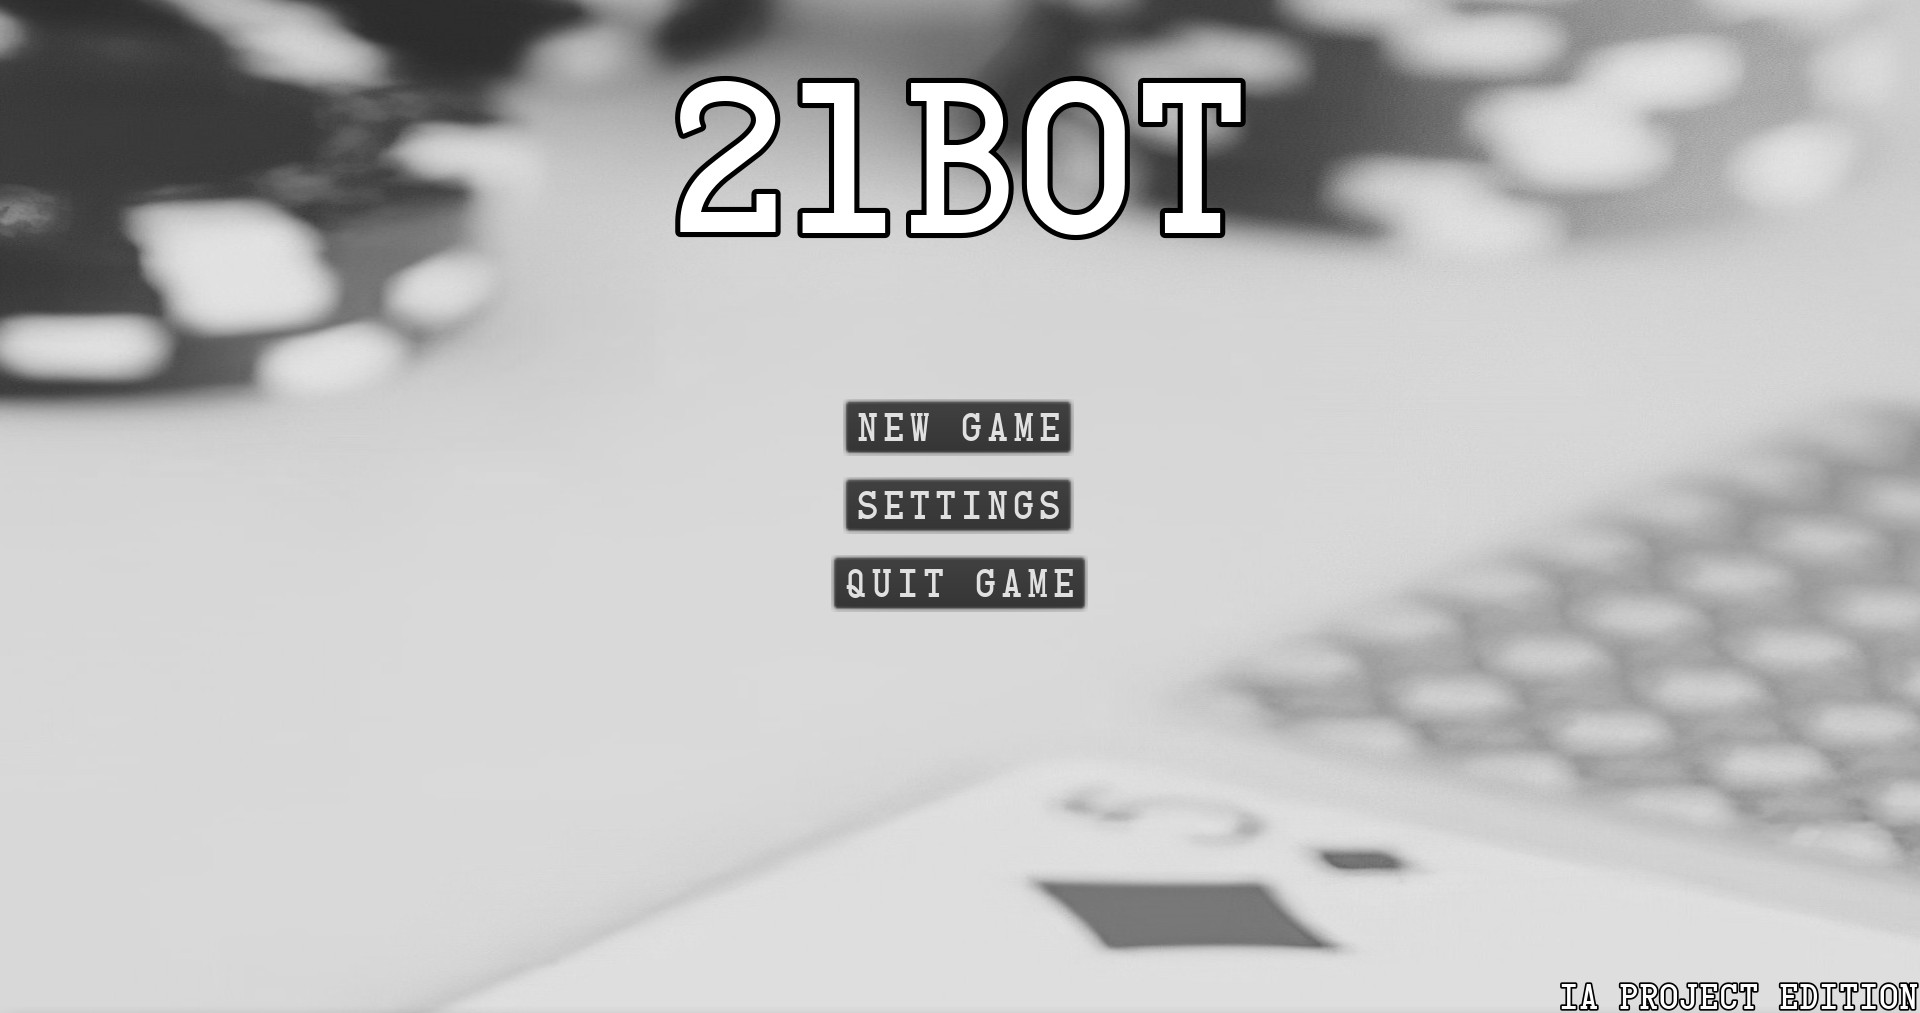
\includegraphics[width=\linewidth]{main_screen.jpg}
    \caption{Tela do menu principal}
    \label{fig:main_menu}
\end{figure}

\newpage

Na figura \ref{fig:main_menu} temos a tela do menu toda vez que o jogador rodar pela 
primeira vez a aplicação. O menu principal possui duas opções que são relevantes: \emph{New game} e \emph{Settings}

\begin{figure}[ht] 
    \centering
    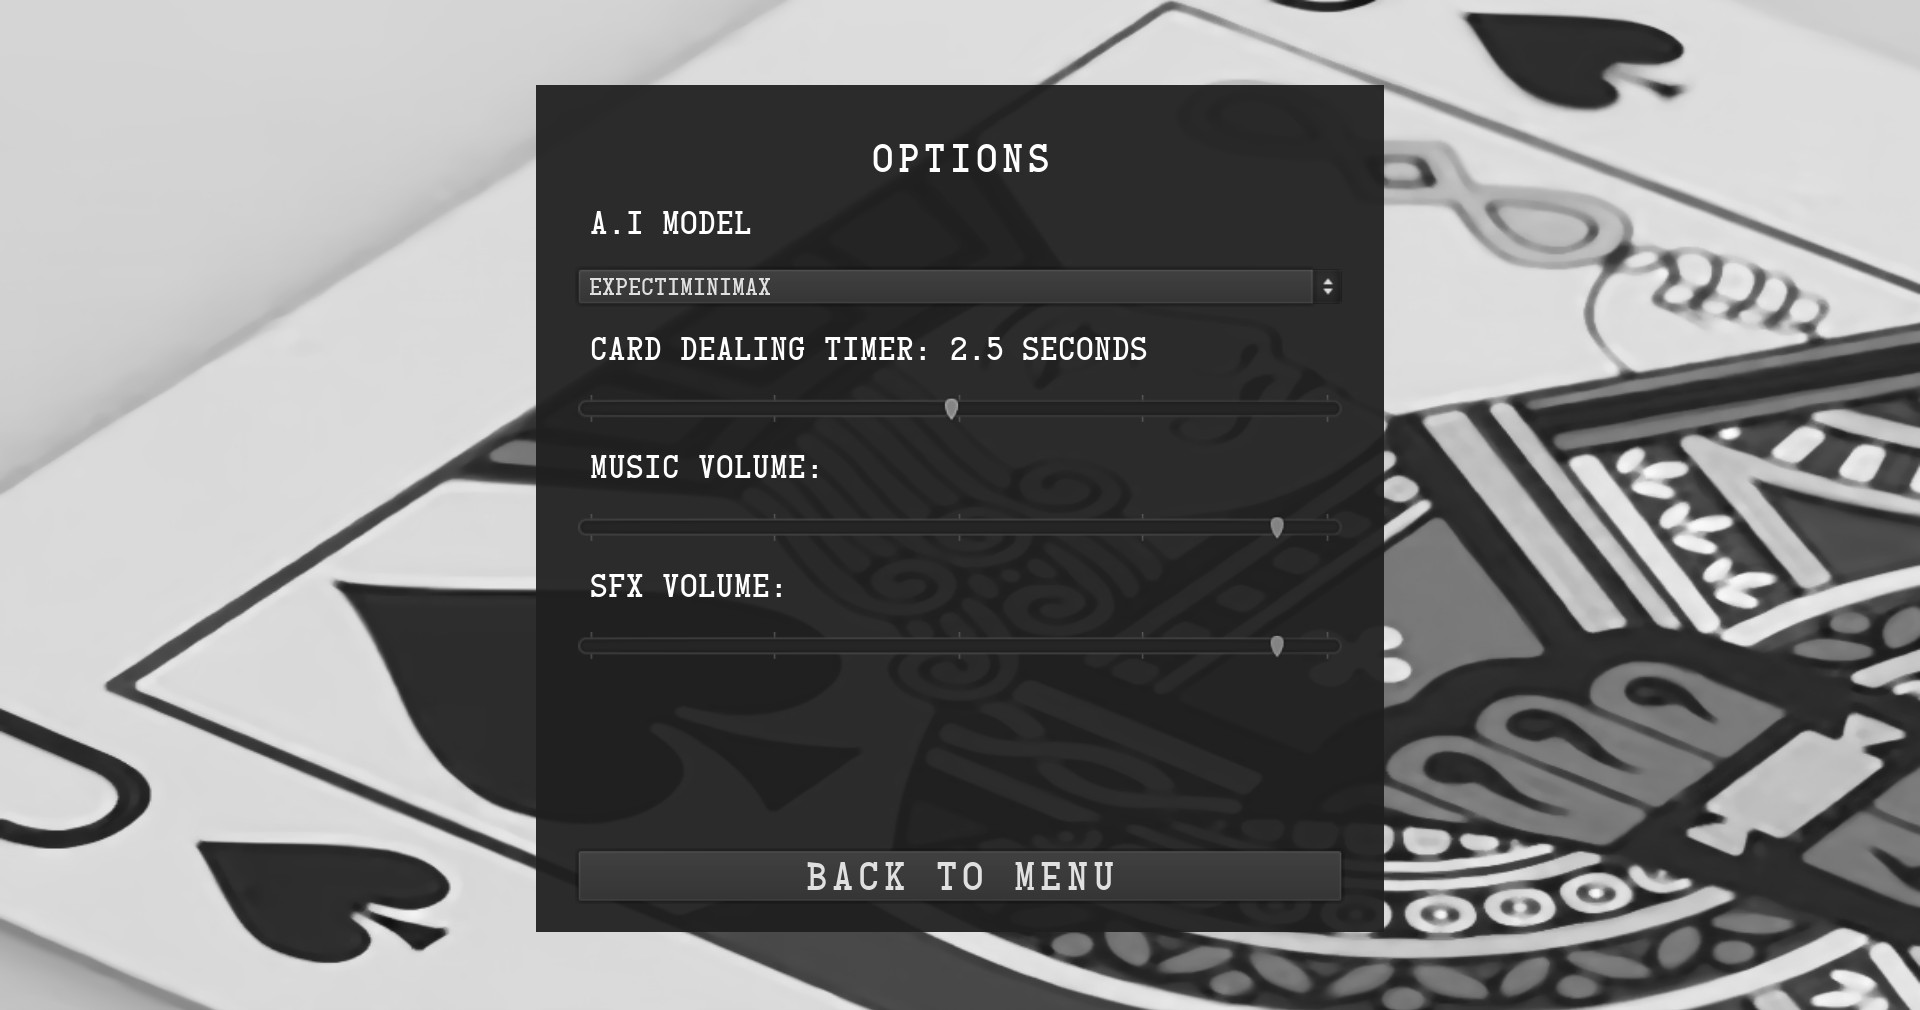
\includegraphics[width=\linewidth]{settings.jpg}
    \caption{Tela do menu de configurações}
    \label{fig:settings}
\end{figure}

Na tela de mostrada na figura \ref{fig:settings} é possível escolher qual será a estratégia 
empregada pelo inimigo, que no caso as opções são: \emph{Expectimax} e \emph{Counting Cards}.

Além disso, é também configurar outras opções do jogo, como o tempo para 
as cartas descerem e o volume do jogo.

Por fim vamos a atração principal, o jogo em si:

\begin{figure}[ht] 
    \centering
    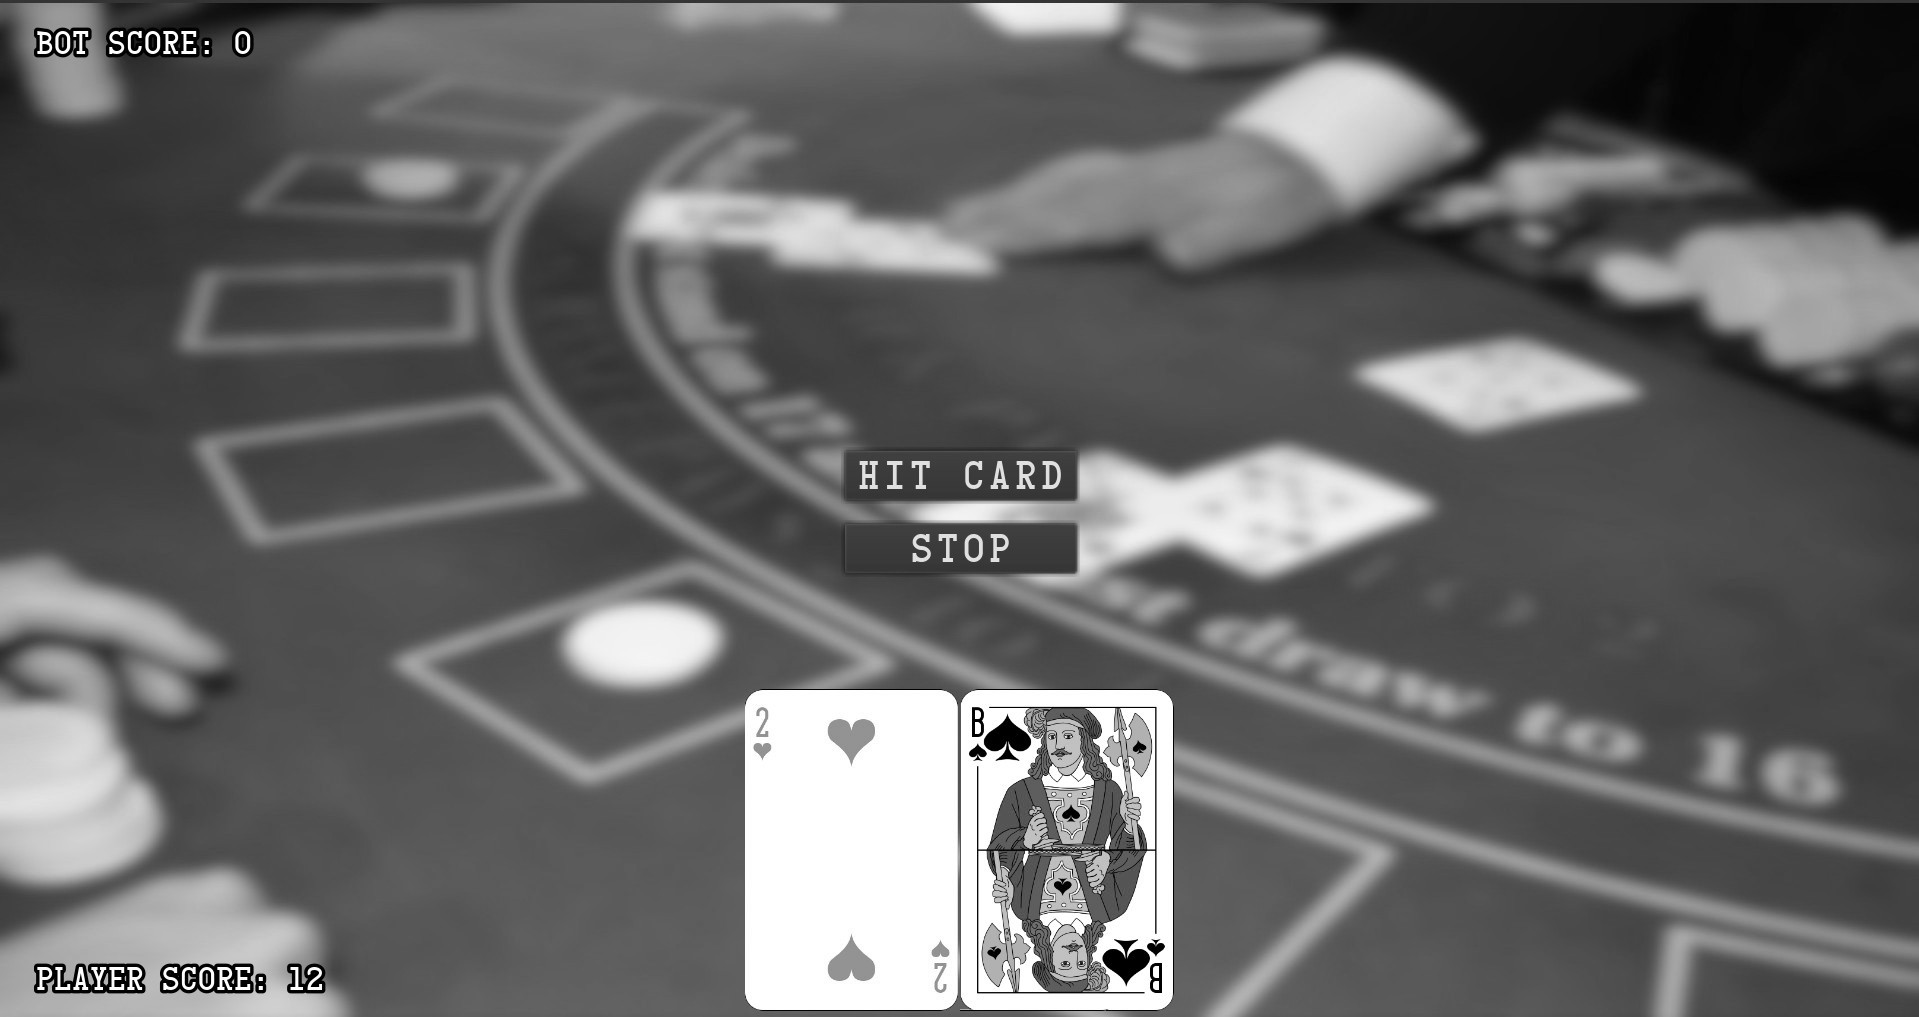
\includegraphics[width=\linewidth]{game.jpg}
    \caption{Tela principal do jogo}
    \label{fig:game}
\end{figure}

Como é possível ver na figura \ref{fig:game}, o jogador (na parte inferior)
da tela, recebe duas cartas, enquanto que o inimigo(Inteligência Artificial)
recebe duas cartas sendo uma delas viradas para cima e a outra para baixo. Em 
outras palavras o inimigo sempre será o dono da mesa(dealer).

Acima das carta, o jogador tem duas opções:
\begin{itemize}
    \item \emph{Hit}: O jogador receberá uma carta, se o jogador ficar com um 
    placar superior a 21 pontos, o jogo irá terminar e a tela de Fim de jogo (Game Over)
    irá aparecer na tela. Caso contrário o jogo irá somar o resultado das cartas ao placar 
    e exibir na tela 
    \item \emph{Stand}: O jogador irá passar seu turno para o oponente e não poderá 
    comprar mais cartas.
\end{itemize}

\begin{figure}[ht] 
    \centering
    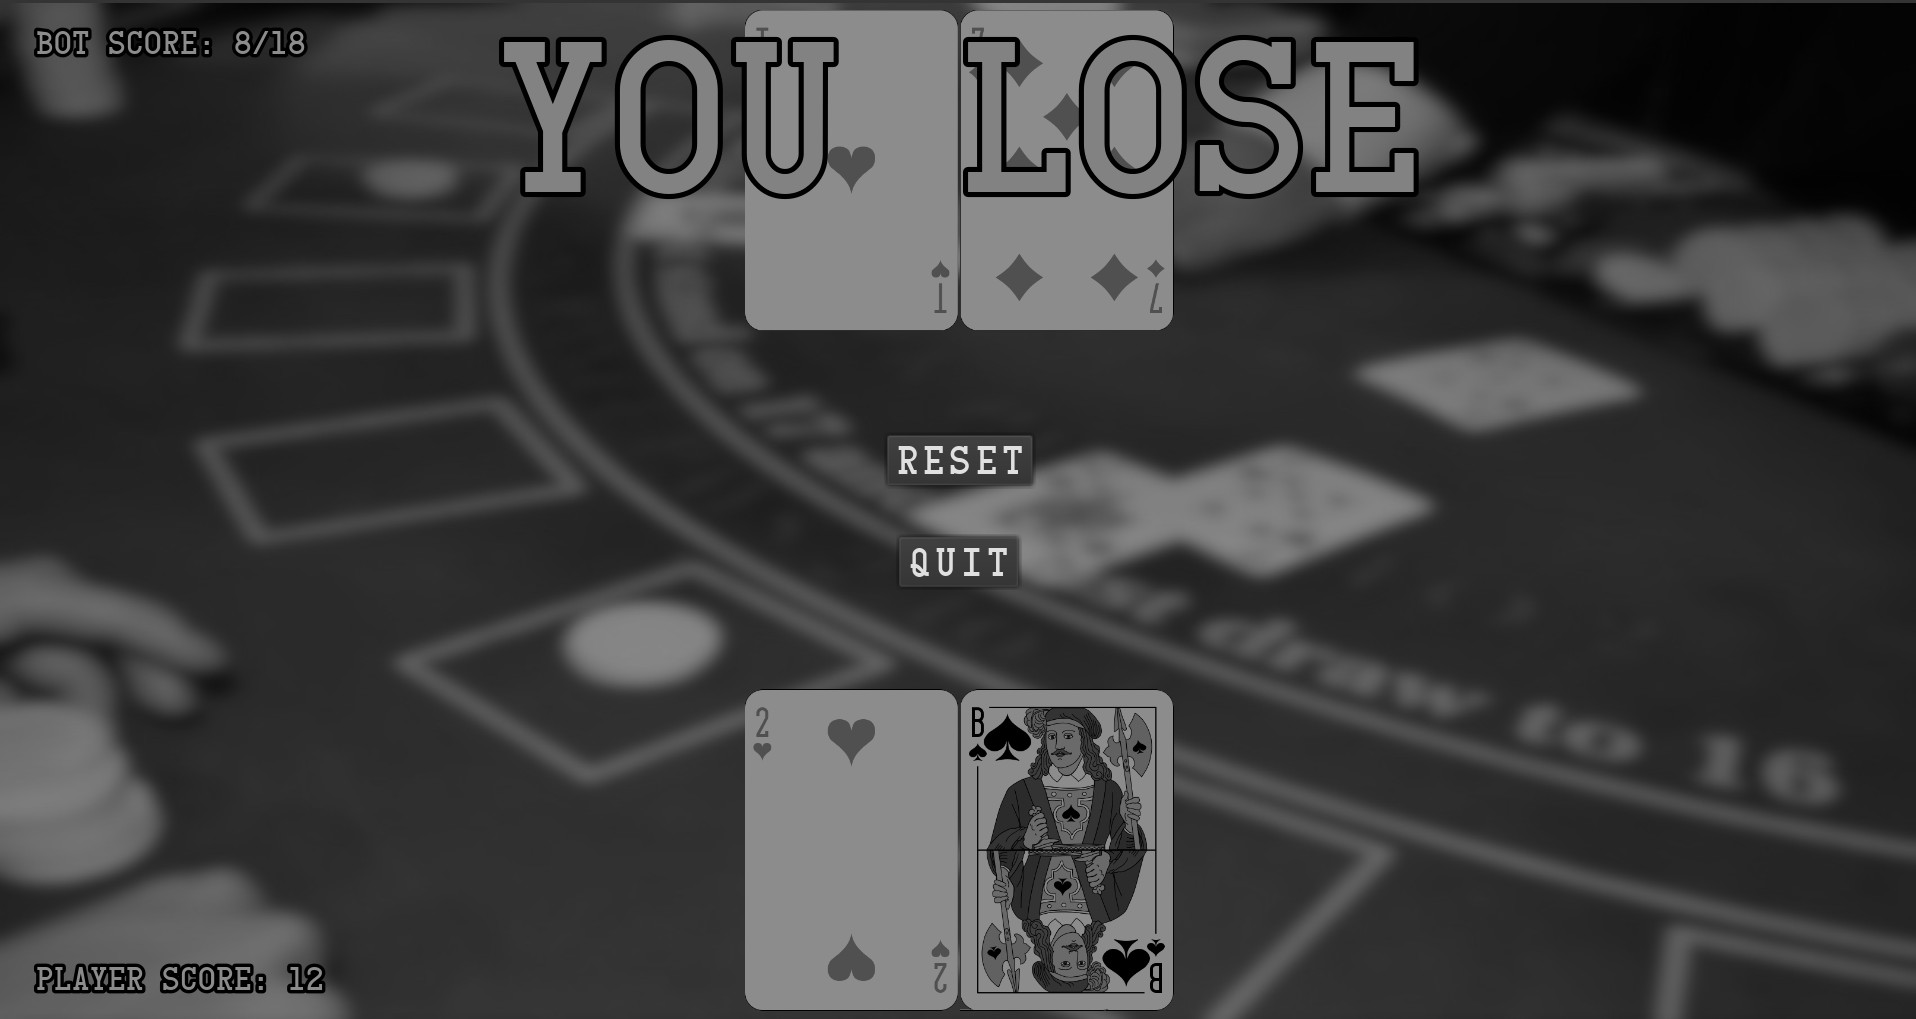
\includegraphics[width=\linewidth]{you_lose.jpg}
    \caption{Tela quando o jogador perde}
    \label{fig:you_lose}
\end{figure}

\begin{figure}[ht] 
    \centering
    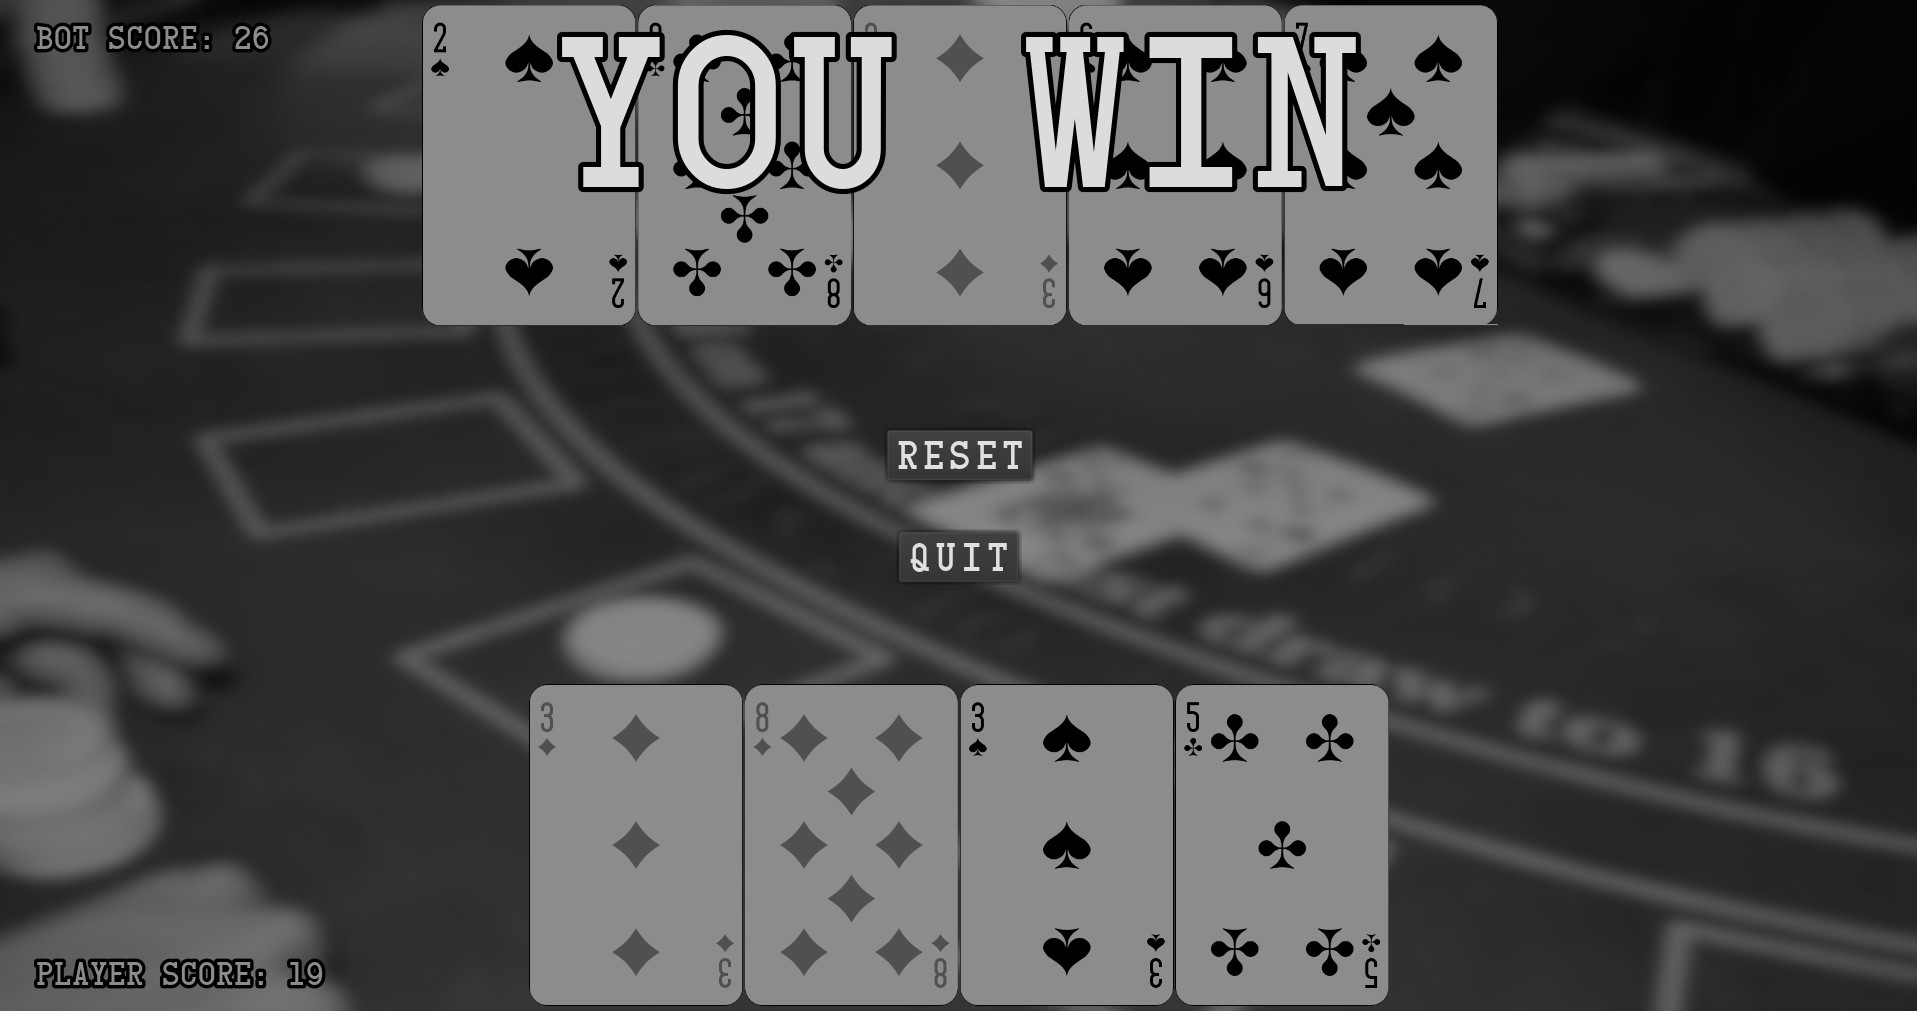
\includegraphics[width=\linewidth]{you_win.jpg}
    \caption{Tela quando o jogador ganha}
    \label{fig:you_win}
\end{figure}

\newpage 

\subsection{Testes}

A maneira em como foi realizado os testes, foi a partir do teste manual 
de cinquenta(50), cem(100) e cento e cinquenta(150) testes isolados, feito no total 
trezentos testes(300) com o intuito de analisar a precisão das diferentes estratégias 
e analisando a porcentagem de vitória de cada uma das políticas. Por fim, foi também 
analisado o tempo de execução das funções.

\begin{table}[htbp]
    \centering
    \caption{Precisão das políticas}
    \begin{tabular}{|c | c | c | c|} 
        \hline
        Estratégias & \multicolumn{3}{|c|}{\textbf{Porcentagem de vitória por número de testes}} \\ 
        \cline{2-4} 
          & 50 & 100 & 150 \\ 
        \hline
        Contar cartas  & 41.0\% & 41.4\% & 41.9\% \\
        \hline
        Expectiminimax & 38.4\% & 38.6\% & 38.9\% \\
        \hline
    \end{tabular}
    \label{tab:precision}
\end{table}

\begin{table}[htbp]
    \centering
    \caption{Tempo de execução}
    \begin{tabular}{|c | c |} 
        \hline
        Estratégias & Tempo médio de execução (em segundos) \\ 
        \hline 
        Contar cartas  & 0.2 \\
        \hline
        Expectiminimax & 0.8 \\
        \hline
    \end{tabular}
    \label{tab:execution_time}
\end{table}

A partir da análise das tabelas \ref{tab:precision} e \ref{tab:execution_time} 
o Expectimax obteve resultado levemente piores que o algoritmo de contar cartas,
o que pode indicar que a heurística escolhida \cite{Introduction-high-low} \cite{odds-house-edge} \cite{win-loss-data} ou o que o fator de possibilidade não 
foram os melhores , e com mais teste e ajuste poderia a ter resultados melhores que o 
contar cartas. Porém, por causa da sua complexidade e o seu tempo de execução 
sendo consideravelmente maior,o algoritmo do Expectimax neste 
cenários explorados não demonstrou-se uma solução viável para substituir uma técnica bem 
estabelecida como o contar cartas, mas em situações futuras com uma melhor heurística 
talvez em determinados cenários e também com um número mais substancial de testes, pode 
ser que o algoritmo em questão possa demonstra-se viável para uso. 

